% game24 - Solves a game 24 scenario
% Copyright (C) 2020 Tim Gesthuizen <tim.gesthuizen@yahoo.de>
%
% This program is free software: you can redistribute it and/or modify
% it under the terms of the GNU General Public License as published by
% the Free Software Foundation, either version 3 of the License, or
% (at your option) any later version.
%
% This program is distributed in the hope that it will be useful,
% but WITHOUT ANY WARRANTY; without even the implied warranty of
% MERCHANTABILITY or FITNESS FOR A PARTICULAR PURPOSE.  See the
% GNU General Public License for more details.
%
% You should have received a copy of the GNU General Public License
% along with this program.  If not, see <https://www.gnu.org/licenses/>.

\documentclass[11pt,a4paper]{article}
\author{Tim Gesthuizen \and Tom Couperus}
\title{Game 24}
\usepackage{tikz}
\usetikzlibrary{trees,fit,arrows,positioning,shapes}
\usepackage{listings}
\usepackage[a4paper,bindingoffset=0.2in,%
  left=1in,right=1in,top=1in,bottom=1in,%
  footskip=.4in]{geometry}
\usepackage{mathptmx}
\setlength\parindent{0px}
\usepackage{hyperref}
\usepackage{xcolor}
\hypersetup{
    colorlinks,
    linkcolor={red!50!black},
    citecolor={blue!50!black},
    urlcolor={blue!80!black}
}
\usepackage{multicol}
\usepackage{listings}
\usepackage{placeins}
\lstalias{shell}{sh}
\definecolor{comment-green}{rgb}{0,0.6,0}
\definecolor{linenumber-gray}{rgb}{0.5,0.5,0.5}
\definecolor{string-mauve}{rgb}{0.58,0,0.82}
\lstset{
  backgroundcolor=\color{white},
  basicstyle=\footnotesize,
  breakatwhitespace=false,
  breaklines=true,
  captionpos=b,
  escapeinside={\%*}{*)},
  extendedchars=true,
  frame=single,
  keepspaces=true,
  numbers=left,
  numbersep=5pt,
  rulecolor=\color{black},
  showspaces=false,
  showstringspaces=true,
  showtabs=false,
  stepnumber=5,
  tabsize=4,
  title=\lstname
}
% colors
\lstset{
  commentstyle=\color{comment-green},
  keywordstyle=\color{blue},
  numberstyle=\tiny\color{linenumber-gray},
  stringstyle=\color{string-mauve}
}
\newcommand{\code}[1]{\texttt{#1}}

\begin{document}

\maketitle

\tableofcontents

\listoffigures

\clearpage

\section{Working environment}

In order to collaboratively work together, the following tools were
used:

\begin{description}
\item[Git] As a version control system to handle the C source code for
  the program and the \LaTeX source code for the report.
\item[\LaTeX] To write the report in.
\item[CMake] Is used to build the program and automate testing of the
  software. CMake simplifies the handling of multiple release and
  debug builds of the software.
\item[GCC] As the primary C compiler to target.
\item[Clang] As the secondary C compiler to check the code does not rely
  on GCC-only features. Clang is known to be more strict about what is
  allowed by the language standards.
\item[tcc] As a third, more minimalistic C compiler that does not fall
  into the ``GCC / GCC compatible'' category. It also aided in
  checking whether all optional GCC features are correctly excluded
  from the compilation when they are not available\footnote{See for
    example the usage of \code{\_\_builtin\_unreachable()}, which is
    available in Clang and GCC, in section~\ref{sec:src}.}.
\end{description}

It was decided to share results via \url{github.com}. The main version
of the repository, which contains the merged results, is hosted at
\url{https://github.com/tgesthuizen/game24}.
In order to not publish proprietary software, the files in the
publicly visible repository have been licensed under the GPL3+.

\section{Problem description}

A program shall be written that solves the \textit{Game of 24}.
In this game you are given 4 numbers and need to come up with a
selection of the 4 arithmetic operators $+$, $-$, $\cdot$ and $\div$ to
reduce these numbers to the number 24.
The numbers can be rearranged in any order and the order of the
operations can also be manipulated.
See figure~\ref{fig:trees} for examples of syntax trees.

\input{tikz/syntax-trees.inc}
\input{tikz/syntax-tree-construction.inc}

\section{Problem analysis}
\label{sec:analysis}

The problem is to construct all possible syntax trees and evaluate
them systematically.
Selecting the operators is not difficult:
There is a set $Operators = \{+, -, \cdot, \div\}$. Generate all
permutations of a multi-set $M$ such that $\vert M \vert = 3$.
\newcommand{\complexop}{{\vert Operators \vert}^3}
\newcommand{\opconnect}{4 \cdot 3 \cdot 3 \cdot 2 \cdot 2 \cdot 1}
This results in $\complexop$ combinations of
operators.

To create a syntax tree from the four operands and the three operators
the following algorithm is used:
Move the seven nodes of the tree into an array, where the four
numbers are placed in front of the three operators.
Now construct an arena from which the operator inputs can be
choosen. The initial bounds of the arena are $[0, 4)$.
The first operator to ``wire up'' will be array entry 4, at the end
of the arena.
Then repeat the following steps for all operators:
\begin{enumerate}
  \item Connect the left hand side of the operator with one of the
    elements in the arena. Swap the selected element to the last
    element in the arena and move the end of it one spot to the left.
  \item Connect the right hand side of the operator with one of the
    elements in the arena. Swap the operator with the selected
    operand. This is done as the operator is now fully connected and
    can be used as an input for the following operators.
\end{enumerate}
At the end of this algorithm the first
element of the array will always be the root node of the tree. In the
implementation the last swap is omitted so that the root node of the
tree is always the last node.
In the implementation the operators use indices into the array to
refer to their left and right hand side operands. This means that
swapping the actual elements of the array will break the referencing
of the operator nodes.
Therefore an extra indirection is used where the indices of the real
nodes are stored in an array and only the indices in this
array are swapped.
Through this indirection it is possible to virtually swap elements in
the array without changing the physical arrangement of the nodes in
memory.
Find an example of this algorithm in figure~\ref{fig:treecon}.

Given this algorithm the total number of different syntax tree
``forms'' is $\opconnect$.
Given the amount of operators, there are $\complexop \cdot \opconnect = 9216$
different syntax trees that need to be checked.

\section{Design of the first iteration of the program}

The user enters the four numbers the program will try to find solutions
for. The program then calculates all permutations and builds up the
syntax trees for them. If a syntax tree evaluates to 24, it is
printed.
It should be noted that all of this can be done in $\mathcal{O}(1)$
space.
The above requirements result in the following software parts:
\begin{enumerate}
\item \code{main} and user interactions
\item Syntax tree creation and permutation
\item Syntax tree evaluation
\item Syntax tree printing
\end{enumerate}

\section{Problems with the first iteration}

The first iteration of the program does very well. On Tim Gesthuizens
laptop the program takes a little bit longer than a tenth of a second
to run.
Surprisingly, as is shown in section~\ref{sec:opt1}, GCC is able to
fold most of the code into the \code{main} function.
Even the indirect call of \code{iterateAllSyntaxTrees} to
\code{checkAndPrintCallback} is detected and inlined.
As shown in section~\ref{sec:perf1}, the hottest part of the program
is the evaluation of syntax trees.
As expected the compiler was not able to inline the two recursive
functions that traverse the binary trees, therefore they are quite
slow.
As the time spent in \code{evalSyntaxTree} is only around $50\%$,
the maximal speedup possible by optimizing it is around $\times 2$.

Although the first iteration of the program does what it is intended to do,
it does so in a very ugly way. As an example, the output for the numbers $2$ $2$ $3$ $9$
is:
\begin{multicols}{2}
\begin{verbatim}
((2 * 9) + (2 * 3))
((2 * 3) + (2 * 9))
((2 * 9) + (3 * 2))
((3 * 2) + (2 * 9))
((2 * 3) + (9 * 2))
((9 * 2) + (2 * 3))
((2 * 9) + (2 * 3))
((2 * 3) + (2 * 9))
((2 * 3) + (2 * 9))
((2 * 9) + (2 * 3))
((3 * 2) + (2 * 9))
((2 * 9) + (3 * 2))
((2 * 3) + (2 * 9))
((2 * 9) + (2 * 3))
((9 * 2) + (2 * 3))
((2 * 3) + (9 * 2))
((3 * 2) + (2 * 9))
((2 * 9) + (3 * 2))
((3 * 2) + (9 * 2))
((9 * 2) + (3 * 2))
((2 * 9) + (3 * 2))
((3 * 2) + (2 * 9))
((9 * 2) + (3 * 2))
((3 * 2) + (9 * 2))
...
\end{verbatim}
\end{multicols}

While these are unique solutions to a computer they look like the same
solution to a human. This is because the computer does not know about
the associativity and commutativity of the $+$ and $\cdot$
operations.

This issue can be solved in two ways:
\begin{enumerate}
\item \label{opt:rewrite} Rewrite part of the generation routine to
  omit redundant trees
\item \label{opt:filter} Filter the trees after the generation for
  duplicates
\end{enumerate}

Option \ref{opt:rewrite} might be the faster version, but it has
several drawbacks:
\begin{itemize}
\item It makes the already complex code for tree generation more
  complex
\item The \code{iterateAllSyntaxTrees} function does one thing,
  adding another thing (filtering) would violate the single
  responsibility principle.
  This function should be changed when there is a change to how trees
  are generated, not when new shortcuts in evaluation are discovered.
\end{itemize}

Therefore option \ref{opt:filter} will be implemented in the second iteration.

\section{Implementing a filter for duplicate solutions}

The second iteration of the program shall solve the main problem of
the first iteration:
Printing trees that are equivalent by means of associativity
and commutativity.
This problem is divided into two subproblems:
\begin{description}
\item[Canonicalization] Transform equivalent trees into equal trees.
  This part shall be implemented by the function
  \code{canonicalizeTree}.
\item[Hashing] Collision free hashing of tree structures allows space
  efficient checking for duplicates.
  This function shall be implemented by the function
  \code{hashTree}.
\end{description}

The callback function shall be extended in the following way:
\begin{enumerate}
\item The current tree shall be checked whether it evaluates to 24.
\item If this is the case the tree is canonicalized using
  \code{canonicalizeTree}.
\item Next, the hash of the canonicalized tree is calculated using
  \code{hashTree}.
\item A binary search through the hashes of all previously printed
  trees is done to see whether an equivalent tree has already been
  printed.
\item If an equivalent tree hasn't already been printed, the current tree
  is printed and the hash is added to the array of previously printed
  arrays.
\end{enumerate}

\subsection{Canonicalization}

In order to transform all equivalent trees into the same tree, an
ordering for equivalent trees needs to be introduced.
This way a tree can be transformed into the smallest or largest tree
in the ordering.
This kind of problem is well known in compiler theory.
An interesting property of it is that while the trees need to be ordered, 
the ordering itself is not important.

As the program stores the array nodes in a contiguous array, each node
has an associated index. This property is used to order them.
All trees that are equivalent by means of associativity can be transformed
into the same tree by sorting the operand indices of associative nodes.
See figure~\ref{fig:assoccanon} for an example.
This can be extended to commutativity by storing all operands of
adjacent commutative and associative nodes in a list and sorting the
list at the end.
See figure~\ref{fig:commutcanon} for an example.
In addition, if the operand indices of non-commutative operators are
not ordered, the operands and indices need to be swapped.
Otherwise trees with non-commutative operators might be printed
multiple times just because of a different layout in memory of the
same tree.

\subsection{Hashing}

Hashing trees using a collision free algorithm allows more storage
efficient comparison of trees. 
It is important to note that only trees whose result is 24 need to be used, 
since only those trees are relevant to the problem.
Each tree has 3 operators and 4 numbers. Since there are 4 unique operators, 
each operator can be represented by a 2 bit pattern. 
The 4 numbers are not stored, since they are the same across all trees. 
The differences between trees are the operands of each operator, so these are stored. 
Specifically, the index of each operand. 
By using the same arena principle as at tree construction (see figure~\ref{fig:treecon}), it is 
possible to represent this value with 2 bits, since the size of the arena will at most be 4. 

\section{Analysis of the second iteration}

The second iteration is capable of canonicalizing trees so that
equivalent trees become equal trees.
Afterwards these trees can be efficiently hashed to form a set of
already seen trees.
This allows the program to only print one version of a set of
duplicate trees.
To name a negative point, the addition to the program is quite large.
The amount of source code more than doubled in comparison to iteration
one.
In addition the program lost its $\mathcal{O}(1)$ space efficiency.
It now requires a heap allocation in order to store the set of already
seen trees.
On the other hand there are quite few elements in the set for a
typical run of the program and the small hash size of 16~bits keeps
the expense of this addition small.
It might even be possible to calculate a small enough maximum of set
entries so that the set could be stored on the stack, regaining the
$\mathcal{O}(1)$ space efficiency.
As in the first iteration, the most cpu cycles are spend in the
\code{evaluateSyntaxTree} function.
The new branch of code execution does not add significant runtime
cost \footnote{See section \ref{sec:perf2}}.
On systems with slower I/O operations it might even be faster because
of the smaller program output.

Because of difficulties implementing the changes it was decided to add
some basic unit tests for part of the operations. The unit test suite
is by no means comprehensive, it just aided in analyzing bugs that
were discovered in development versions of the program.
The authors discovered that unit testing in C is not as easy and
productive as expected and not a low hanging fruit as in other
languages which have better support for adding higher level
abstractions.
Assertions were also added in order to partially test whether
invariants that cannot be managed by abstractions in C are kept up and
hold.

This second version is the first version of the program where
compilers have more varying output: Clang and GCCs inliner work
differently and decided to emit calls to functions at different
points. As implied, this means that both compilers decide to
emit some the functions and not to inline everything into the main
function apart from recursive tree traversing functions.
The assembly output has grown to $\sim 1000$ lines. On one hand, this
shows that the code generated by the compilers is still quite dense,
on the other hand this indicates that abstractions could not be used
well to reuse existing concepts.

\section{Summary}

Both iterations have their own value:
While the first iteration is fully functional with only 200 lines of
code, the second iteration seems less redundant to humans and shows
solutions that seem less duplicate to a human.
One optimization is missed by iteration two: One could transform
subtractions to additions of negative numbers and divisions to
multiplications of fractions.
This would allow to divide the whole tree into only commutative
chunks, as only additions and multiplications are left.
After normal canonicalization fractions and negative numbers could be
transformed back.
This would allow for even better results.

Using C for the implementation was a particular challenge.
A lot of ideas cannot be represented in syntax. Invariants cannot be
enforced. C's domain is programming for very restricted environments
or when absolute control is required of what is happening.
This is not the case here and other languages would have a been a lot
more capable of expressing the concepts and algorithms.
Large parts of the program have been prototyped in C++ and Scheme and
have been translated into C afterwards.
Implementing the program in C caused a lot of headaches that could
have been prevented by using a different language.
The source code could be easily shrinked into a fourth of its size if
it were written in a different language.

\begin{figure}[h]
  \centering
  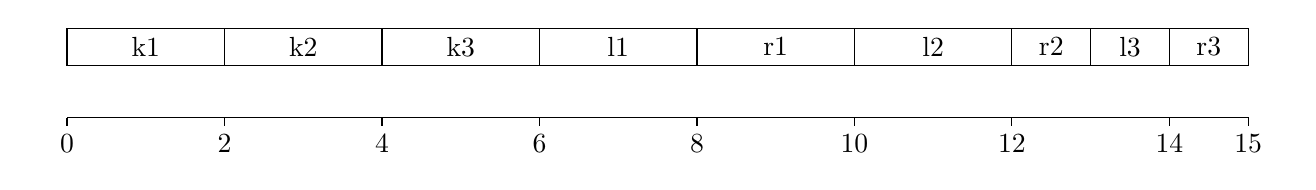
\begin{tikzpicture} [
    box/.style={draw,%
      outer sep=0,%
      align=center},
    bitc/.style={outer sep = 0,
      minimum width= 1cm,
      align = center}
    ]
    \node[box, minimum width=2cm] (h0) {k1};
    \foreach \i/\size/\name [remember=\i as \lastx (initially 0)] in {1/2cm/k2,2/2cm/k3,3/2cm/l1,4/2cm/r1,5/2cm/l2,6/1cm/r2,7/1cm/l3,8/1cm/r3} 
        \node[box, minimum width=\size, right= 0mm of h\lastx] (h\i) {\name};
    \node[bitc, below = 1cm of h0.west] (b0) {0};
    \draw (b0.north) -- +(0,.1);
    \foreach \i [remember=\i as \lasti (initially 0)] in {2,4,6,...,14} {%
      \node[bitc, right = 1cm of b\lasti] (b\i) {\i};
      \draw (b\i.north) -- +(0,.1) -- +(-2,.1);
    }
    \node[bitc, below = 1cm of h8.east] (b15) {15};
    \draw (b15.north) -- +(0,.1) -- + (-1,.1);
  \end{tikzpicture}
  \begin{description}
    \item[k?] Kind of operator \textit{?}.
    \item[l?] Left hand side operand index for operator \textit{?}.
    \item[r?] Right hand side operand index for operator \textit{?}.
  \end{description}
  \caption{Bit layout of a compressed tree in memory}
  \label{fig:comptree}
\end{figure}

\input{tikz/commutative.inc}

\FloatBarrier
\clearpage
\huge{Measurements and source code}
\addcontentsline{toc}{section}{Measurements and source code}
\input{measurements.inc}
\section{Source code}
\label{sec:src}
\subsection{First iteration}

\lstinputlisting[language=C]{iteration1.c}

\subsection{Second iteration}

\lstinputlisting[language=C]{game24.c}

\end{document}
